\documentclass[11pt,a4paper,onecolumn]{article}
\usepackage[left=2cm,text={17cm,24cm},top=2.5cm]{geometry}
\usepackage[czech]{babel}
\usepackage[utf8]{inputenc}
\usepackage{times}
\usepackage{graphicx}
\usepackage{float}
\usepackage{picture}
\usepackage{setspace}
\onehalfspacing
\begin{document}
\begin{titlepage}
  \begin{center}

    \textsc{\Huge Vysoké učení technické v~Brně\\\huge Fakulta informačních technologií}\\
    \vspace{\stretch{0.382}}\LARGE Databázové systémy\\\Huge
    Dokumentace projektu\vspace{\stretch{0.618}}\\
  \end{center}
  {\Large\today\hfill Daniel Klímaj, Vojtěch Večeřa }
\end{titlepage}
\section{Úvod}
Přiložený skript vytváří objekty databáze, reprezentující systém na správu CVT zařízení na FIT. Koncept se s~kládá z~9 tabulek, 1 sekvence, 2 triggerů, 2 procedur, 1 materializovaného pohledu a 1 indexu. Tabulky a vazby mezi nimy vychází ze zadání z~projektu zadaného vrámci předmětu Softwarové inženýrství. 

\section{Pokročilé objekty}
Cílem projektu do Databázových systému bylo realizovat konceptuální návrh v~Oracle databázi a vytvořit některé pokročilé objekty databáze a pochopit jejich použití a význam. 
\subsection{Triggery}
První trigger byl použit pro ověření rodného čísla zaměstnance a je zavolán před vložením záznamu do příslušné tabulky. Tento trigger vrací 3 různé chybové kódy (20001, 20002, 20003) v~případě, že bylo zadáno nevalidní rodné číslo. Jedná se indikaci nedělitelnosti 11, konečným trojčíslým 000 a špatná reprezentace reálného datumu narození. Druhý trigger slouží pro generování primárního klíč tabulky přesunů k~dosažení této funkcinality je využita sekvence, která slouží jako počítadlo použité pro generování unikátních klíčů.
\subsection{Procedury}
Dalším použitým objektem jsou procedury. První byla použita pro přidávání záznamů do tabulky přesunů s~tím, že jsme ověřili zda osoba žádající o~přesun je za toto zařízení momentálně zodpovědná a může tedy žádat o~jeho přesun. Z~této procedury mohou vzejít 2 chybové kódy (20004, 20005) indikující chyby v~datech žádosti. Druhá procedura slouží k~zjištění kolik zaměstnanců bychom mohli do kterého oddělení přijmout. Parametr procedury slouží ke specifikování kolik zaměstnanců chceme v~odděleních celkem mít. Informace o~současném počtu není implicitně uvedena v~databázi, ale lze ji získat dotazem spojujícím zaměstnance skrze místnosti s~odděleními a využitím agregační funkce \textit{COUNT}. Pro realizaci tohoto dotazu byl využit kurzor, který v~sobě ukládá data získaná dotazem, z~něhož je posléze vytvořena kolekce dat. Ta reprezentuje strunkturu, kterou lze cyklicky procházet a přistupovat k~uloženým prvkům. V~cyklu jsou vypočítány deficity zaměstnanců a následně vytvořeny výstupní zprávy infromující, ve kterém oddělení chybý kolik zaměstnanců.
\subsection{Pohled}
Materializovaný pohled slouží jako přehled, kdo zastává v~systému, kterou funkci. Takovýto pohled slouží ke snížení zátěže na databázi, pokud předpokládáme, že tato data budou často vyžadována. Pohled je aktualizován vždy, když někdo požádá o~data v~něm uložená. Data jsou aktualizována pokud byla přidána nová data do obsažených tabulek. Dotaz na pohled je méně náročná operace než dotaz do více tabulek a filtrování dat z~nich na základě podmínek a vazeb.\newpage
\subsection{Index}
V~aplikaci byl vytvořen index poruchy na sloupci \textit{k\_oprave} a technik tabulky \textit{Porucha}. Pro realizaci takovéhoto indexu je většinou využit B-strom, který umožňuje rychlejší přístup k~záznamům s~hledanými daty oproti případu, kdy index není použit nám pomáhá například s~urychlením dotazů dotazujících se na informace ohledně jednotlivých oprav nebo techniků.
\section{Optimalizace}
Pro demonstraci optimalizace byl zvolen dotaz:

\begingroup
\leftskip8ex
\rightskip\leftskip
{\ttfamily\noindent SELECT z.jmeno, z.prijmeni, p.k\_ oprave, COUNT(*) as Pocet\_ poruch  \newline FROM Zamestnanec z, Porucha p \newline WHERE z.zamID = p.technik \newline GROUP BY p.k\_ oprave, z.jmeno, z.prijmeni;}\par
\endgroup

Rozdíl mezi zpracováním s~indexem a bez indexu byl zjištěn pomocí funkce \textit{EXPLAIN PLAN}, která
vypisuje jednotlivé kroky potřebné k~provedení dotazu. Z~analýzy pomocí \textit{EXPLAIN PLAN} jsme zjistili, že je v~obouch případech je nutné provést 5 operací k~získání požadovaného výsledku. První čtyři operace jsou stejné poslední oprace se liší.

\bigskip
Operace:
\begin{enumerate}
\item SELECT STATEMENT
\item HASH (GROUP BY)     
\item HASH JOIN
\item TABLE ACCESS (FULL)
\item TABLE ACCESS (FULL) / INDEX (FULL SCAN)
\end{enumerate}

Rozdíl je zde v~tom, že zatím co \textit{TABLE ACCESS (FULL)} prohledává pokaždé celou tabulku jako takovou, kdežto  \textit{INDEX (FULL SCAN)} hledá shodu pouze procházením záznamu uložených v~indexu pro vyhledávané informace. Jedná se tedy o~podstatně jednodušší a rychlejší operaci. Čím víc unikátních hodnot v~indexovaném sloupci máme tím efektivnější index v~porovnání ve vyhledávání bez indexu

To nám reflektuje cena operace, která se nám sníží ze 3 na 1, což odpovídá snížení
vstupně-výstupní ceny a ceny za procesor. Pokud bychom měli v~v~tabulce \textit{Porucha} více
položek tak bychom došli k~podstatně větším rozdílům co se náročností těch dvou operací týče, ale
i na tomto příkladu je dopad optimalizace znatelný.\newpage

\section{Entity relationship diagram}
\begin{figure}[H]
\begin{centering}
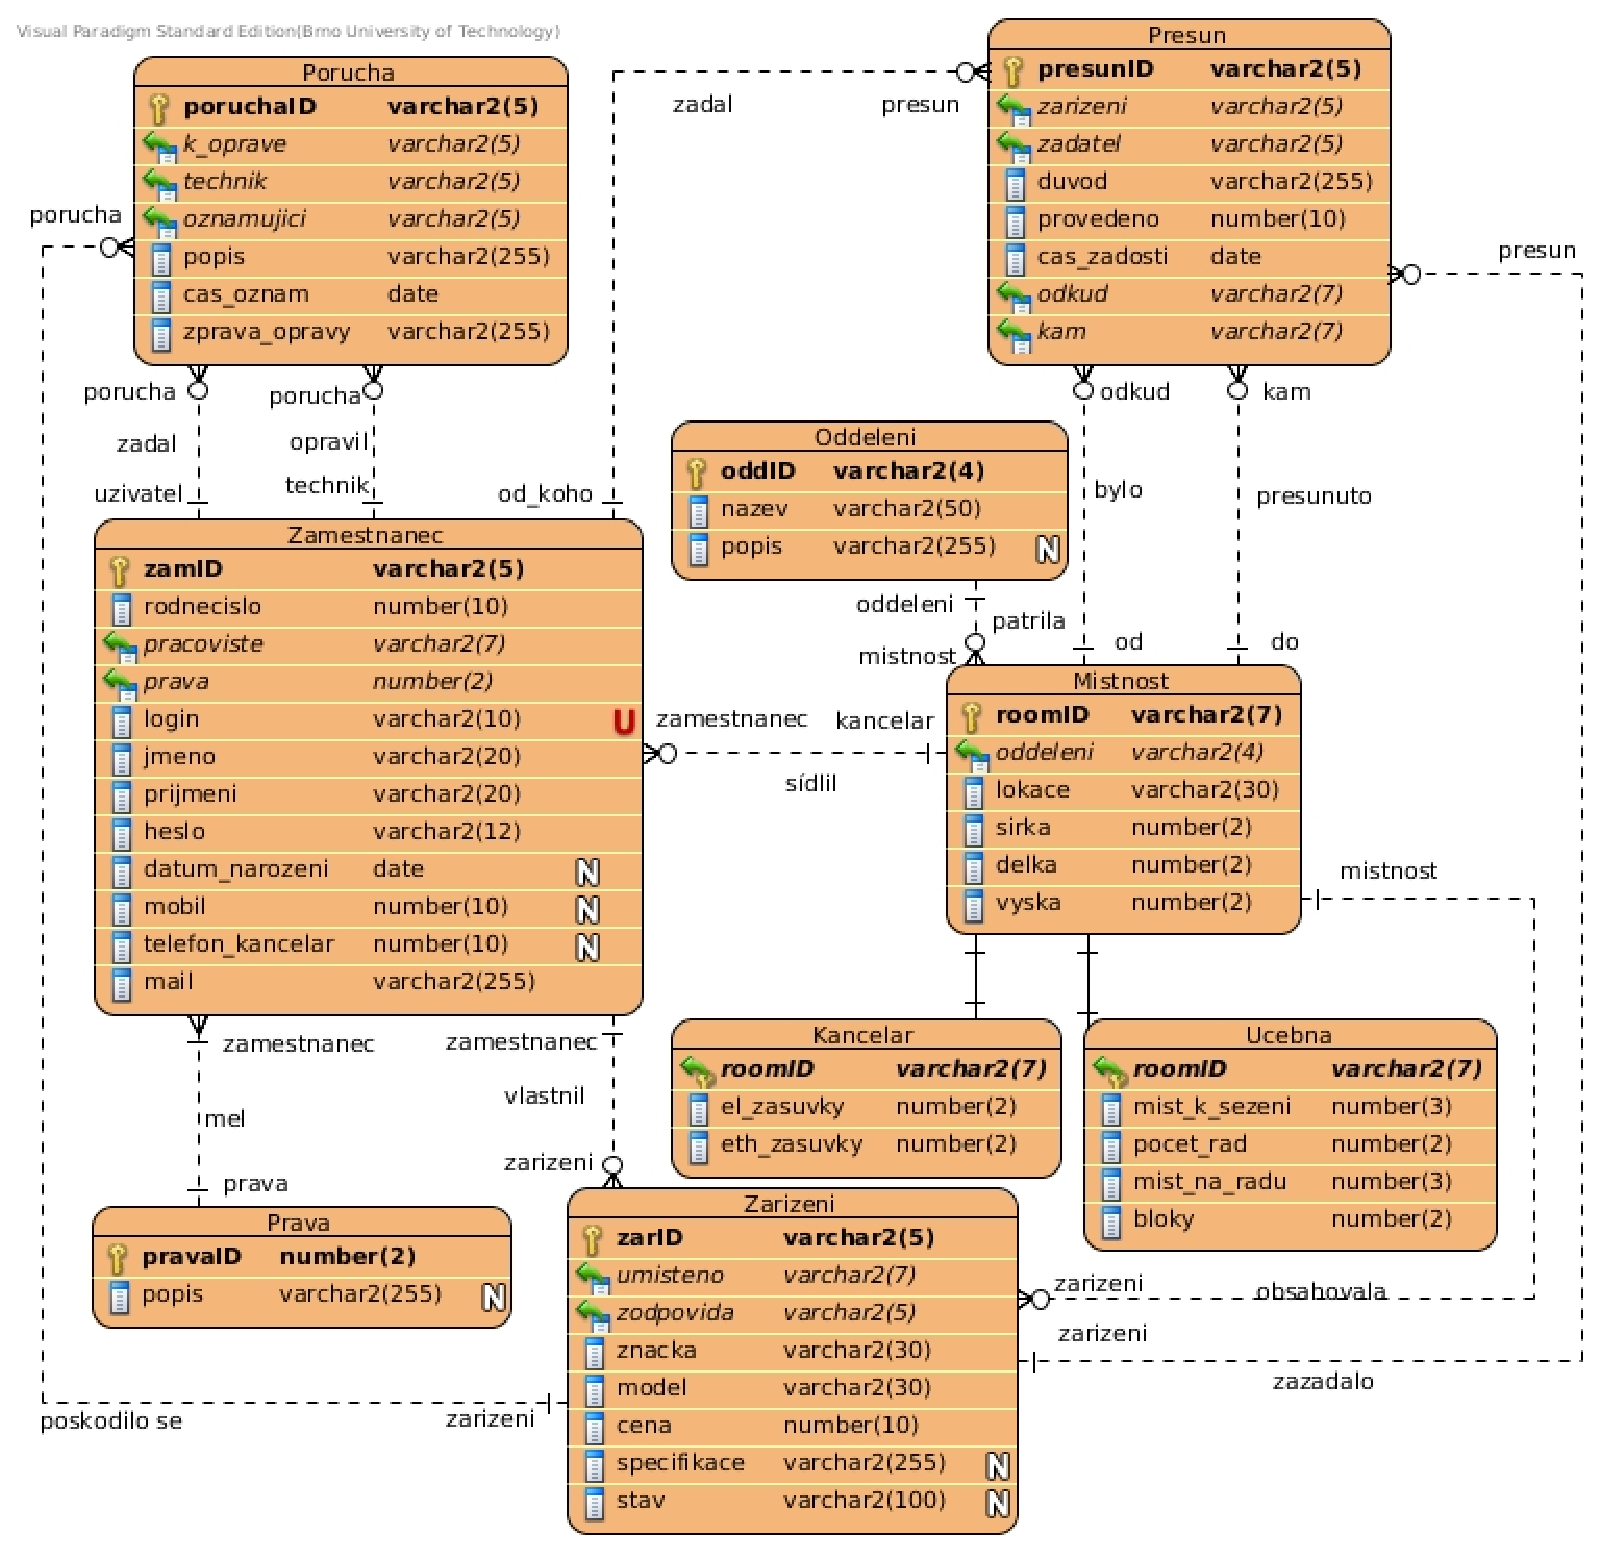
\includegraphics[scale=0.63]{./diagrams/proj4ERD.eps}
\end{centering}
\end{figure}
\newpage
\section{Diagram případů užití}
\begin{figure}[H]
\begin{centering}
\includegraphics[scale=0.49]{./diagrams/proj4UC.eps}
\end{centering}
\end{figure}
\end{document}